\chapter{Inyección de fallos}
\label{ch:InyeccionDeFallos}

\lettrine[lraise=-0.1, lines=2, loversize=0.2]{L}{a} inyección de fallos es una
técnica que permite recrear los efectos que produce la radiación sobre un
circuito. Esta técnica es ampliamente usada ya que permite estudiar en qué parte
de un circuito causa más efecto un error lógico y qué partes son más resistentes a
este tipo de error. El diseño de circuitos destinados a trabajar en entornos 
hostiles, donde recibirán altas dosis de radiación ionizante, encuentra en esta
técnica una gran ayuda, ya que permite estudiar la sensibilidad de sus módulos a
este tipo de errores sin necesidad de fabricarlo y testearlo bajo radiación real.
Con esto se acelera enormemente el proceso de diseño y refuerzo de circuitos
resistentes a radiación.

En nuestro caso, hemos empleado técnicas de inyección de fallos como ayuda para el
diagnóstico de \gls{SEU}, es decir, tratar de localizar el error, determinar en 
qué biestable (\textit{\gls{FF}}) se ha producido la conmutación lógica y durante
qué ciclo de reloj ha ocurrido. El papel de la técnica en el diagnóstico es el de
recrear los efectos que tendrían \gls{SEU} concretos sobre el circuito, de forma
que podamos generar una base de datos donde tener relacionados cada localización
espacial y temporal de un error lógico con su consecuencia a la salida del
circuito. Esta base de datos, en diagnóstico de \gls{SEU}, toma el nombre de
diccionario de fallos, y se obtienen mediante campañas de inyección de fallos.

Durante una campaña de inyección de fallos se ejecuta el \gls{CUT} con las mismas
señales de entrada una y otra vez, partiendo siempre desde el reset. En cada
ejecución, se inyecta un fallo en alguno de las posibles localizaciones (\gls{FF}, 
ciclo). Si el \gls{CUT} está formado por \textit{"n"} \gls{FF} y las pruebas se 
ejecutan durante \textit{"m"} ciclos de reloj, existirán \textit{"n·m"} posibles 
combinaciones donde inyectar un error lógico.

% Imagen 1 -> Ejecución de una camapaña de inyección de fallos.
\begin{figure}[htbp]
    \centering
    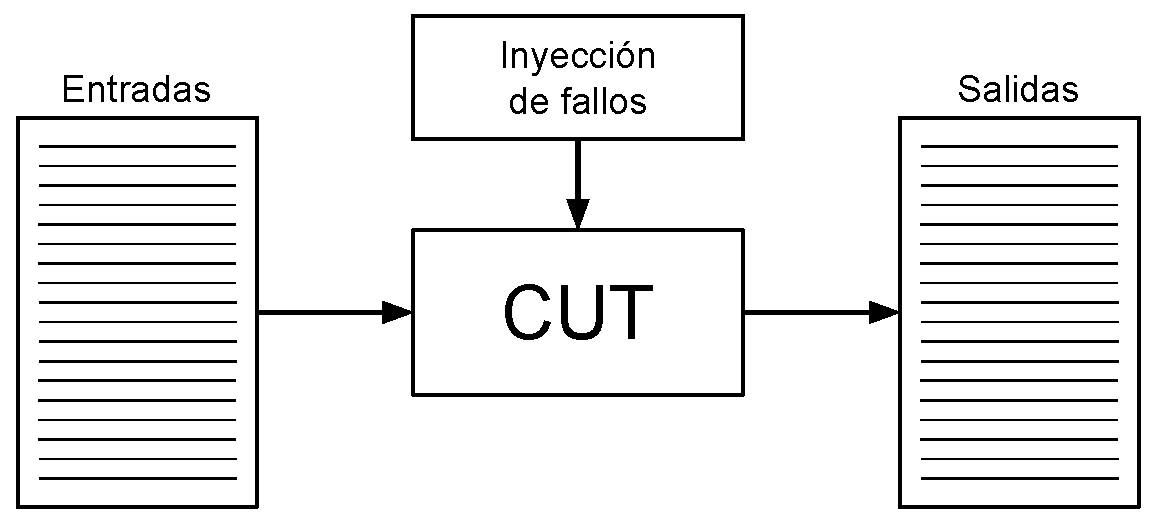
\includegraphics[width=0.95\linewidth]
    {InyeccionDeFallos/figuras/fig31.pdf}
    \caption{Ejecución de una campaña de inyección de fallos}
    \label{fig:Inyeccion}
\end{figure}

Las salidas que se obtienen, ciclo a ciclo, durante una ejecución de la campaña, 
se registran y almacenan junto con la información de la inyección que las ha 
causado. Dado que solo nos interesan los errores, no que se traten de ceros cuando
deberían ser unos o viceversa, la salida del circuito (entendiendo "salida" como 
el conjunto de las salidas de los ciclos que dura la prueba) es comparada bit a 
bit con la salida que se obtendría si no existiese fallo alguno. Para llevar a 
cabo esta comparación se emplea la operación lógica \textit{XOR}, ya que por
definición, toma el valor 1 únicamente cuándo sus entradas son distintas.

% Imagen 2 -> Postprocesado de la salida de una ejecución de la campaña.
\begin{figure}[htbp]
    \centering
    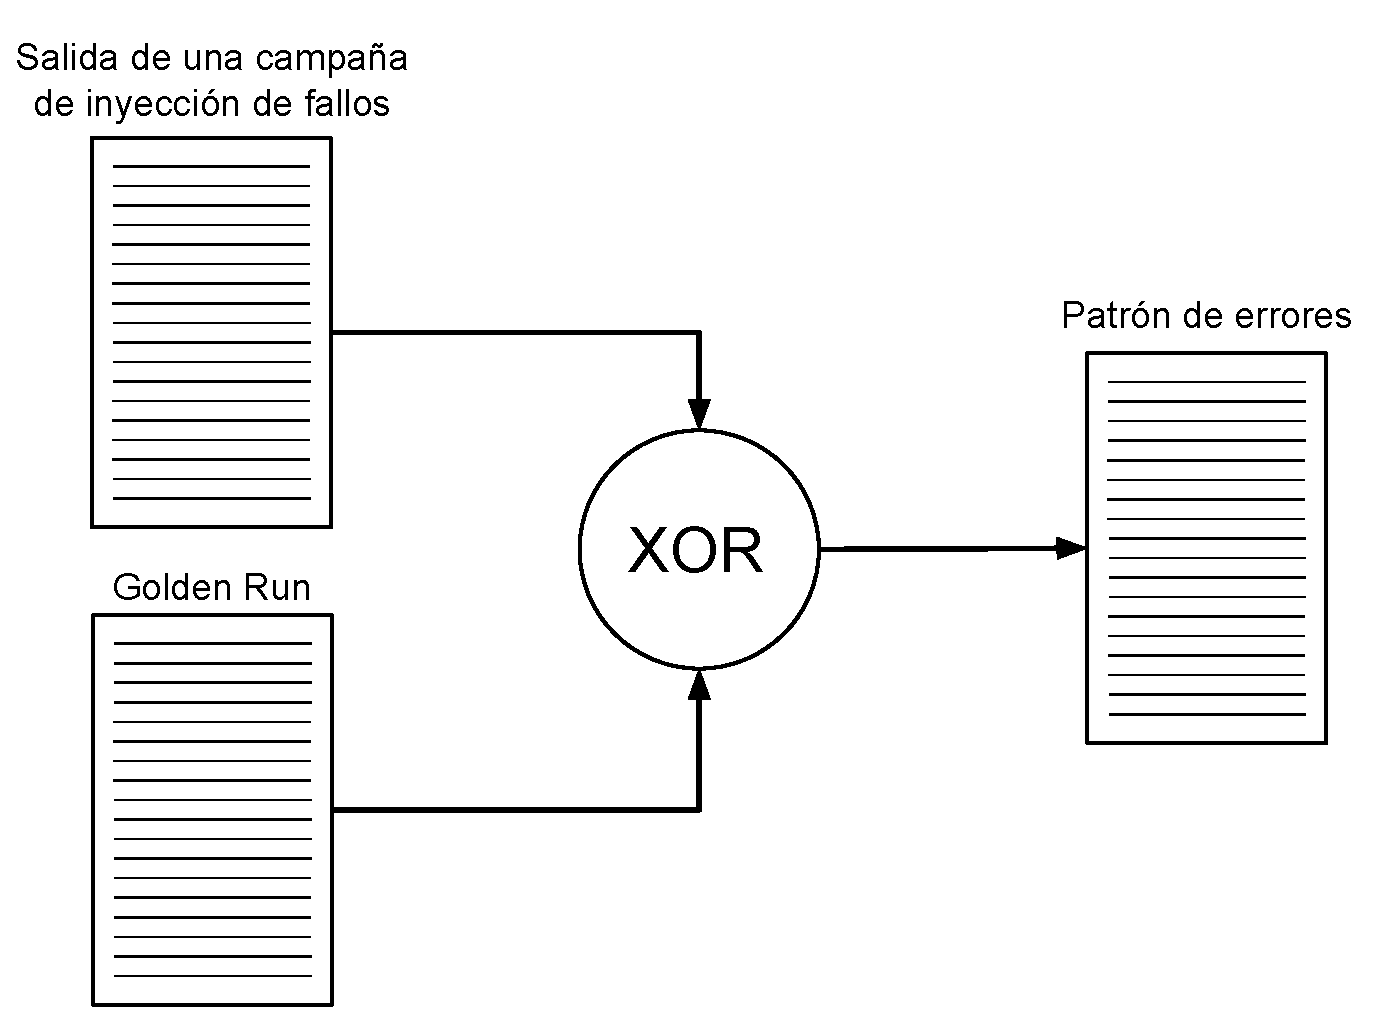
\includegraphics[width=0.95\linewidth]
    {InyeccionDeFallos/figuras/fig32.pdf}
    \caption{Postprocesado de la salida de una ejecución de la campaña}
    \label{fig:PostprocesadoSalida}
\end{figure}

% Definir run -> como XOR de golden run y las salidas -> discrepancias
Aplicandola para cada correspondiente pareja de bits entre una salida de la 
campaña y la salida del circuito sin inyecctar, conseguimos resaltar los errores
que causa el \gls{SEU} inyectado. A esta versión de la salida de una ejecución de
la campaña donde solo toman valor lógico alto los errores causados por la
inyección nos referiremos de ahora en adelante como \textit{"Run"}. Así mismo, a 
la salida del circuito durante una ejecución libre de inyecciones la denominaremos
\textit{"Golden Run"}.
% Definir golden run (arriba)

% Definir entrada del diccionario
Cada run, junto con la información de la inyección que lo ha causado, constituye
una entrada del diccionario. Es decir, cada entrada del diccionario está formado
por la localización del \gls{SEU} recreado (\gls{FF}, ciclo) y las discrepancias 
que ha causado a la salida. El diccionario estará constituido por tantas entradas 
como inyecciones se hayan realizado durante la campaña.

% Diccionario de fallos completo o exhaustivo
Se dice que el diccionario de fallos es completo o exhaustivo cuando se genera a
partir de una campaña de inyección de fallos exhaustiva, es decir, se inyectan
todas las posibles combinaciones de \gls{FF} y ciclo. 
% Campaña exaustiva --> tiempo necesario para generarla n*m*m
Como hemos visto, existen \textit{"n·m"} inyecciones posibles. Además, cada una de 
las ejecuciones tiene una extensión de \textit{"m"} ciclos, lo que hace un total 
de  \textit{"n·m·m"} ciclos totales de ejecución necesarios para completar una
campaña exhaustiva.

% Inviabilidad de obtener diccionarios exhasutivos en circuitos grandes
La extensión de cada una de las ejecuciones de una campaña, en ciclos, debe ser
tal que el error lógico inyectado tenga el tiempo suficiente para producir un 
patrón de salidas identificable y diferenciable del resto de inyecciones. Si el
circuito es pequeño, estas diferencias se harán notables de forma más temprana.
Cuando el circuito tiene un número de \gls{FF} elevado, el número de ciclos
necesario para que los patrones de salida se diferencien lo suficiente unos de 
otros, y por tanto, podamos identificar distintos \gls{SEU}, también lo es. Esto
hace que ejecutar una campaña de inyección de fallos exhaustiva, y por tanto, 
obtener un diccionario de fallos exhaustivo sea inviable para circuitos grandes.

% Diccionario de fallos incompleto o no exhaustivo
Cuando esto sucede, no queda más opción que la de trabajar con diccionarios de
fallos incompletos. Las campañas de inyección de fallos no exhaustivas pueden
enfocarse a un subconjunto de biestables del circuito, limitar las inyecciones en 
tiempo, o realizarse de forma aleatoria. El diccionario de partida con el que
hemos diagnosticado en circuitos grandes es incompleto y aleatorio, aunque
plantearemos también el uso de diccionarios específicos para subconjuntos de
\gls{FF} y ciclos en otras fases del diagnóstico cuándo la primera no es
suficiente.

% El estudio realizado parte de la premisa de que la plataforma de inyección de
% fallos está bien diseñada y funciona correctamente.
Es importante destacar que el estudio aquí realizado requiere de una plataforma 
de inyección de fallos que funcione correctamente. La verificación del correcto 
funcionamiento de esta plataforma no es ámbito de esta investigación.

\section{FT-Unshades2}
\label{sec:FT-Unshades2}
Esta es la plataforma de inyección de fallos con la que hemos trabajado durante
toda la investigación. Fué diseñada por un equipo del departamento de Ingeniería
Electrónica de la Universidad de Sevilla en el año 2011 \cite{FTU} y ha sido
utilizada por multitud de equipos para el desarrollo de sus proyectos, incluidos
algunos pertenecientes a la Agencia Espacial Europea (\textit{\acrshort{ESA}}).

Está basada en las \acrshort{FPGA} (\textit{\acrlong{FPGA}}) avanzadas de
\textit{Xilinx}. Concretamente, hace uso de una de sus características, llamada
\textit{"Capture and ReadBack"}, mediante la cual tienen acceso a partes del
esquema de configuración. De esta forma pueden realizar cambios de valor en 
cualquier registro de usuario.

Partiendo de esta funcionalidad de las tarjetas de \textit{Xilinx} consiguen
controlar todo el proceso de inyección. Manejan la señal de reloj precisamente
para poder inyectar en el ciclo y biestable deseado de forma que el \gls{CUT} no
sea capaz de percibir el proceso de inyección.

\vspace{0.3cm}
\textit{"FTU2 puede ser una de las plataformas de inyección de fallos basada en 
hardware más poderosas que existe para la evaluación de \gls{SEE}. La flexibilidad
y recursos disponibles hacen a FTU2 apropiada para diferentes usos, no solo como
emulador de hardware para técnicas de inyección de fallos"}.
\vspace{-0.2cm}
{\flushleft{\hfill \emph{- J. M. Mogollon, H. Guzmán-Miranda, J. Nápoles, J. 
Barrientos, M. A. Aguirre, 2011, pág. 5} \cite{FTU}}}
\vspace{0.3cm}

La plataforma FTU2 tiene potencia y flexibilidad suficiente para llevar a cabo
todos las labores de inyección de fallos que se han necesitado para este trabajo.

\endinput
